\section{Introduction}
\label{sec:intro}

\begin{figure*}[t]
\centering
\IfFileExists{figures/fig1_comem_autofigure.pdf}
  {
\includegraphics[width=0.96\textwidth]{figures/fig1_comem_autofigure.pdf}}
  {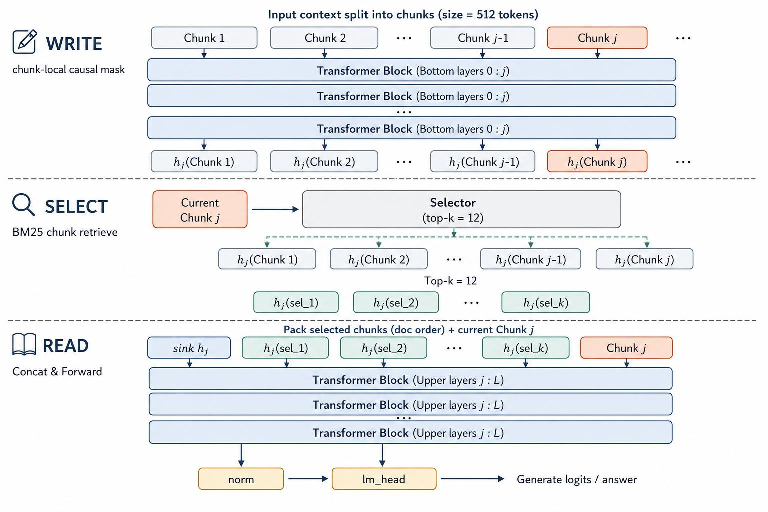
\includegraphics[width=0.96\textwidth]{figures/Structure.pdf}}
\caption{\textbf{CoMem turns transformer depth into a cross-query reuse axis.}
\textsc{Write} prepays layers $[0{:}j)$ once per document chunk,
\textsc{Select} retrieves a bounded working set, and \textsc{Read} resumes
$[j{:}L)$ with the query present. The matched $j{=}0$ endpoint uses the same
selected chunks, order, sink, mask, and adapter while replaying all layers,
thereby isolating the incremental depth effect. Overlap-Write supplies a small
amount of left document context without enlarging the stored object or Read
pack.}
\label{fig:teaser}
\end{figure*}

Long-context applications repeatedly ask new questions about the same manuals,
repositories, histories, or document collections. Raw-text retrieval reduces
the number of online tokens, but every selected token still traverses every
transformer layer~\citep{rag,xu2024retrievallong}. Reusable-context systems move
this work offline: CacheBlend, TurboRAG, EPIC, APE, and related systems cache
layer-wise KV and repair context or position dependencies
~\citep{cacheblend,turborag,epic,ape,cachecraft}. Yet these interfaces largely
fix what is stored and how much model depth has already been executed. This
leaves a basic systems question unanswered: \emph{how much transformer depth
should each reusable document object prepay?}

We answer this question with \textbf{CoMem}, which exposes the split $j$ between
offline document processing and online query processing. \textsc{Write} runs
each chunk through layers $[0{:}j)$ and stores its residual $h_j$.
\textsc{Select} retrieves top-$k$ chunks. \textsc{Read} packs the selected
residuals with the query and executes only $[j{:}L)$ with full cross-pack
attention. The $j{=}0$ endpoint stores token IDs and replays the identical pack
through all layers. Varying $j$ therefore trades persistent bytes and
write-once computation against per-query model depth while holding retrieved
evidence fixed.

Prior activation-reuse methods cache a chosen intermediate representation for
repeated downstream runs~\citep{readonce,embeddingrecycling}; LLMCache maintains
per-layer activation banks and semantically matches similar inputs at arbitrary
layers~\citep{llmcache}; HCache stores hidden states across layers to reconstruct
layer-wise KV~\citep{hcache}; and PIC/modular-cache systems store or learn
layer-wise KV objects~\citep{cacheblend,epic,kvpacket,cartridgesbase}. CoMem's
specific conjunction is a persistent document object at one chosen split,
direct decoder-suffix continuation, and an identical-evidence $j{=}0$ endpoint.
This formulation makes prepaid depth directly measurable rather than an
implementation constant.

The matched result establishes a clear quality--latency trade-off. On
Qwen3-8B, moving from $j{=}0$ to $j{=}12$ reduces selected-pack Read from
931.9 to 664.4\,ms, a $1.403\times$ speedup, while the paired 15-cell RULER
macro changes from 99.19 to 96.07 (gap 3.12, 95\% CI $[2.36,3.93]$). A
rank-32 self-distillation adapter makes the split interface effective while
leaving the backbone frozen. When bounded selection and depth reuse are
combined, the store-ready 128k online-prefill point falls from 71.37 to
1.10\,s ($64.9\times$); a separate same-adapter, Write-inclusive pipeline
improves from 6.035 to 2.202\,s ($2.74\times$). These measurements answer
different questions: $1.403\times$ isolates prepaid depth, $64.9\times$
measures the composed store-ready bounded-read path, and $2.74\times$ includes
the reusable Write in a separate same-platform cohort.

CoMem further provides a unified measurement of a
single-residual reusable object across quality, per-query latency, persistent
storage, one-time Write, and empirical break-even. The residual costs
8\,KiB/token---18$\times$ smaller than full bf16 KV for Qwen3-8B, but much
larger than text. In the write-once serving harness, CPU-pinned storage breaks
even after 8.9--10.9 repeated queries at 32k for generations up to 128 tokens;
at 128k and one generated token, GPU/CPU placement breaks even after
25.8--27.6 queries. The full serving grid extends these measurements to 1M
stored tokens and four generation lengths (Table~\ref{tab:serving-crossover}).

The experiments yield two further scientific findings. First, a
continuous-prefix $h_{12}$ oracle exactly recovers the 3.12-point matched gap,
locating the attainable loss at the reusable Write interface rather than the
capacity of the upper decoder. A $2{\times}2$ context--position factorization
then identifies missing lower-layer document context as the dominant tested
factor on paired 8k/16k multikey instances: full document context raises 92.5
to 100.0, while remapping positions alone lowers it to 88.0. A deployable
32-token overlap reaches 98.5 with unchanged persistent bytes and per-query
Read. Second, the equal-latency comparison shows that efficiency does not
translate into a selector-independent quality advantage. BM25 replay leads
CoMem by 11.56 points, whereas a frozen-BGE replay edge of 1.00 point is
unresolved under hierarchical cell resampling. This negative result identifies
retrieval policy as a first-order coordinate of the same frontier.

\paragraph{Scope.}
Our central claims concern the matched depth axis, measured amortization, and
the tested Write-context mechanism. CoMem targets repeated queries over stable
corpora with open-weight models; the nearest PIC and learned modular-KV systems
use different backbones and measurement boundaries. We therefore pair the
broader conceptual comparison with one same-Qwen3 minimal-faithful
CacheBlend-style experiment rather than transfer unmatched published numbers.
The full set of deployment, generalization, and statistical limits is
consolidated in the dedicated Limitations section.

\paragraph{Contributions.}
\begin{itemize}[leftmargin=1.2em,itemsep=1pt,topsep=2pt]
\item \textbf{A tunable depth-reuse interface.} CoMem stores one residual per
token at split $j$ and directly resumes the decoder suffix, introducing
transformer depth as an explicit axis for reusable-context serving.
\item \textbf{A matched measurement framework.} The $j{=}0$ endpoint isolates
depth reuse from selection and supports paired quality, Read latency,
persistent-storage, Write, and break-even accounting, including a
$1.403\times$ matched Read speedup, a same-backbone full-depth chunk-KV
comparison, and $64.9\times$ store-ready / $2.74\times$ Write-inclusive 128k
operating points.
\item \textbf{Write-side diagnosis and repair.} A continuous-prefix oracle,
context--position factorization, and overlap sweep explain and recover most of
the tested multikey interface gap without enlarging the persistent object or
online Read.
\item \textbf{A selector-aware deployment result.} Equal-latency BM25 and
frozen-dense audits show when extra raw-text evidence dominates and when the
quality difference remains unresolved, sharpening the conditions under which
depth reuse is useful.
\end{itemize}
